\section{XMBulletin\-Board  Class Reference}
\label{classXMBulletinBoard}\index{XMBulletinBoard@{XMBulletin\-Board}}
{\tt \#include $<$XMManagers.h$>$}

Inheritance diagram for XMBulletin\-Board::\begin{figure}[H]
\begin{center}
\leavevmode
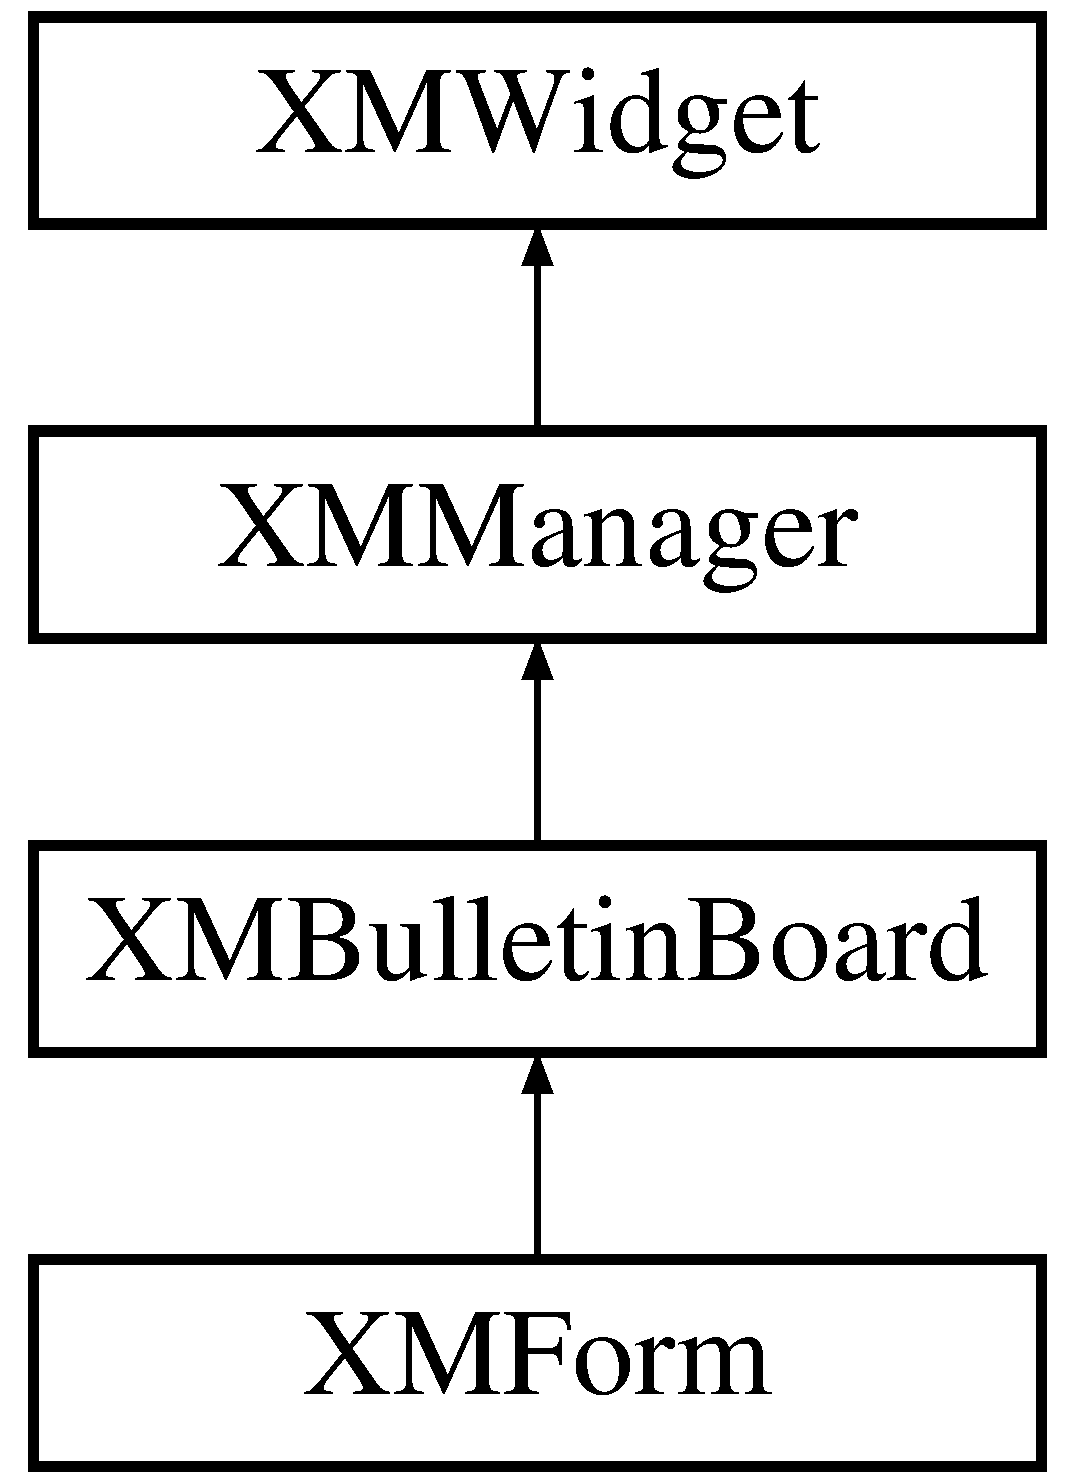
\includegraphics[height=4cm]{classXMBulletinBoard}
\end{center}
\end{figure}
\subsection*{Public Methods}
\begin{CompactItemize}
\item 
{\bf XMBulletin\-Board} (char $\ast$n)
\item 
{\bf XMBulletin\-Board} (Widget w)
\item 
{\bf XMBulletin\-Board} (char $\ast$n, {\bf XMApplication} \&parent, Arg\-List l=NULL, Cardinal num\_\-args=0)
\item 
{\bf XMBulletin\-Board} (char $\ast$n, Widget parent, Arg\-List l=NULL, Cardinal num\_\-args=0)
\item 
{\bf XMBulletin\-Board} (char $\ast$n, {\bf XMWidget} \&parent, Arg\-List l=NULL, Cardinal num\_\-args=0)
\item 
void {\bf Allow\-Overlap} (Boolean allow)
\item 
void {\bf Margins} (Dimension ymargin, Dimension xmargin=0)
\item 
void {\bf Set\-Shadow\-Type} (unsigned char type)
\item 
void {\bf Set\-Abs\-Position} ({\bf XMWidget} \&w, int x, int y)
\end{CompactItemize}
\subsection*{Protected Methods}
\begin{CompactItemize}
\item 
{\bf XMBulletin\-Board} (char $\ast$n, Widget\-Class cl, Widget parent, Arg\-List l, Cardinal num\_\-args)
\end{CompactItemize}


\subsection{Constructor \& Destructor Documentation}
\index{XMBulletinBoard@{XMBulletin\-Board}!XMBulletinBoard@{XMBulletinBoard}}
\index{XMBulletinBoard@{XMBulletinBoard}!XMBulletinBoard@{XMBulletin\-Board}}
\subsubsection{\setlength{\rightskip}{0pt plus 5cm}XMBulletin\-Board::XMBulletin\-Board (char $\ast$ {\em n}, Widget\-Class {\em cl}, Widget {\em parent}, Arg\-List {\em l}, Cardinal {\em num\_\-args})\hspace{0.3cm}{\tt  [inline, protected]}}\label{classXMBulletinBoard_b0}




Definition at line 376 of file XMManagers.h.\index{XMBulletinBoard@{XMBulletin\-Board}!XMBulletinBoard@{XMBulletinBoard}}
\index{XMBulletinBoard@{XMBulletinBoard}!XMBulletinBoard@{XMBulletin\-Board}}
\subsubsection{\setlength{\rightskip}{0pt plus 5cm}XMBulletin\-Board::XMBulletin\-Board (char $\ast$ {\em n})\hspace{0.3cm}{\tt  [inline]}}\label{classXMBulletinBoard_a0}




Definition at line 382 of file XMManagers.h.\index{XMBulletinBoard@{XMBulletin\-Board}!XMBulletinBoard@{XMBulletinBoard}}
\index{XMBulletinBoard@{XMBulletinBoard}!XMBulletinBoard@{XMBulletin\-Board}}
\subsubsection{\setlength{\rightskip}{0pt plus 5cm}XMBulletin\-Board::XMBulletin\-Board (Widget {\em w})\hspace{0.3cm}{\tt  [inline]}}\label{classXMBulletinBoard_a1}




Definition at line 383 of file XMManagers.h.\index{XMBulletinBoard@{XMBulletin\-Board}!XMBulletinBoard@{XMBulletinBoard}}
\index{XMBulletinBoard@{XMBulletinBoard}!XMBulletinBoard@{XMBulletin\-Board}}
\subsubsection{\setlength{\rightskip}{0pt plus 5cm}XMBulletin\-Board::XMBulletin\-Board (char $\ast$ {\em n}, {\bf XMApplication} \& {\em parent}, Arg\-List {\em l} = NULL, Cardinal {\em num\_\-args} = 0)\hspace{0.3cm}{\tt  [inline]}}\label{classXMBulletinBoard_a2}




Definition at line 384 of file XMManagers.h.\index{XMBulletinBoard@{XMBulletin\-Board}!XMBulletinBoard@{XMBulletinBoard}}
\index{XMBulletinBoard@{XMBulletinBoard}!XMBulletinBoard@{XMBulletin\-Board}}
\subsubsection{\setlength{\rightskip}{0pt plus 5cm}XMBulletin\-Board::XMBulletin\-Board (char $\ast$ {\em n}, Widget {\em parent}, Arg\-List {\em l} = NULL, Cardinal {\em num\_\-args} = 0)\hspace{0.3cm}{\tt  [inline]}}\label{classXMBulletinBoard_a3}




Definition at line 388 of file XMManagers.h.\index{XMBulletinBoard@{XMBulletin\-Board}!XMBulletinBoard@{XMBulletinBoard}}
\index{XMBulletinBoard@{XMBulletinBoard}!XMBulletinBoard@{XMBulletin\-Board}}
\subsubsection{\setlength{\rightskip}{0pt plus 5cm}XMBulletin\-Board::XMBulletin\-Board (char $\ast$ {\em n}, {\bf XMWidget} \& {\em parent}, Arg\-List {\em l} = NULL, Cardinal {\em num\_\-args} = 0)\hspace{0.3cm}{\tt  [inline]}}\label{classXMBulletinBoard_a4}




Definition at line 392 of file XMManagers.h.

\subsection{Member Function Documentation}
\index{XMBulletinBoard@{XMBulletin\-Board}!AllowOverlap@{AllowOverlap}}
\index{AllowOverlap@{AllowOverlap}!XMBulletinBoard@{XMBulletin\-Board}}
\subsubsection{\setlength{\rightskip}{0pt plus 5cm}void XMBulletin\-Board::Allow\-Overlap (Boolean {\em allow})\hspace{0.3cm}{\tt  [inline]}}\label{classXMBulletinBoard_a5}




Definition at line 398 of file XMManagers.h.

References XMWidget::Set\-Attribute().\index{XMBulletinBoard@{XMBulletin\-Board}!Margins@{Margins}}
\index{Margins@{Margins}!XMBulletinBoard@{XMBulletin\-Board}}
\subsubsection{\setlength{\rightskip}{0pt plus 5cm}void XMBulletin\-Board::Margins (Dimension {\em ymargin}, Dimension {\em xmargin} = 0)\hspace{0.3cm}{\tt  [inline]}}\label{classXMBulletinBoard_a6}




Definition at line 401 of file XMManagers.h.

References XMWidget::Set\-Attribute().\index{XMBulletinBoard@{XMBulletin\-Board}!SetAbsPosition@{SetAbsPosition}}
\index{SetAbsPosition@{SetAbsPosition}!XMBulletinBoard@{XMBulletin\-Board}}
\subsubsection{\setlength{\rightskip}{0pt plus 5cm}void XMBulletin\-Board::Set\-Abs\-Position ({\bf XMWidget} \& {\em w}, int {\em x}, int {\em y})\hspace{0.3cm}{\tt  [inline]}}\label{classXMBulletinBoard_a8}




Definition at line 410 of file XMManagers.h.

References XMManager::Set\-Constraint().\index{XMBulletinBoard@{XMBulletin\-Board}!SetShadowType@{SetShadowType}}
\index{SetShadowType@{SetShadowType}!XMBulletinBoard@{XMBulletin\-Board}}
\subsubsection{\setlength{\rightskip}{0pt plus 5cm}void XMBulletin\-Board::Set\-Shadow\-Type (unsigned char {\em type})\hspace{0.3cm}{\tt  [inline]}}\label{classXMBulletinBoard_a7}




Definition at line 405 of file XMManagers.h.

References XMWidget::Set\-Attribute().

The documentation for this class was generated from the following file:\begin{CompactItemize}
\item 
{\bf XMManagers.h}\end{CompactItemize}
